\xiaosi

本文提出的方法由三个核心模块组成：基于NCP的Q网络、Double DQN训练框架、以及安全感知的布线拓扑进化搜索。整体架构如下：

环境在每个决策步产生一个运动学观测向量（包含自车和周围4辆最近车辆的位置、速度和朝向共35维特征），经NCP的LTC动力学处理后输出全部神经元的隐状态，再由两层Q-head映射为5个离散动作对应的Q值。智能体以$\varepsilon$-贪心策略选择动作，与环境交互后将转移存入经验回放缓冲区。训练时从缓冲区采样序列，用Double DQN目标更新网络参数。

在此基础上，进化搜索模块对NCP的6个布线参数进行自动优化。搜索过程中，每个候选布线配置被实例化为一个NCP Q网络，快速训练若干步后评估其安全感知适应度，通过选择、交叉、变异迭代优化，最终输出最优布线拓扑。

图\ref{fig:framework}展示了整体框架的数据流和模块关系。

\begin{figure}[H]
    \centering
    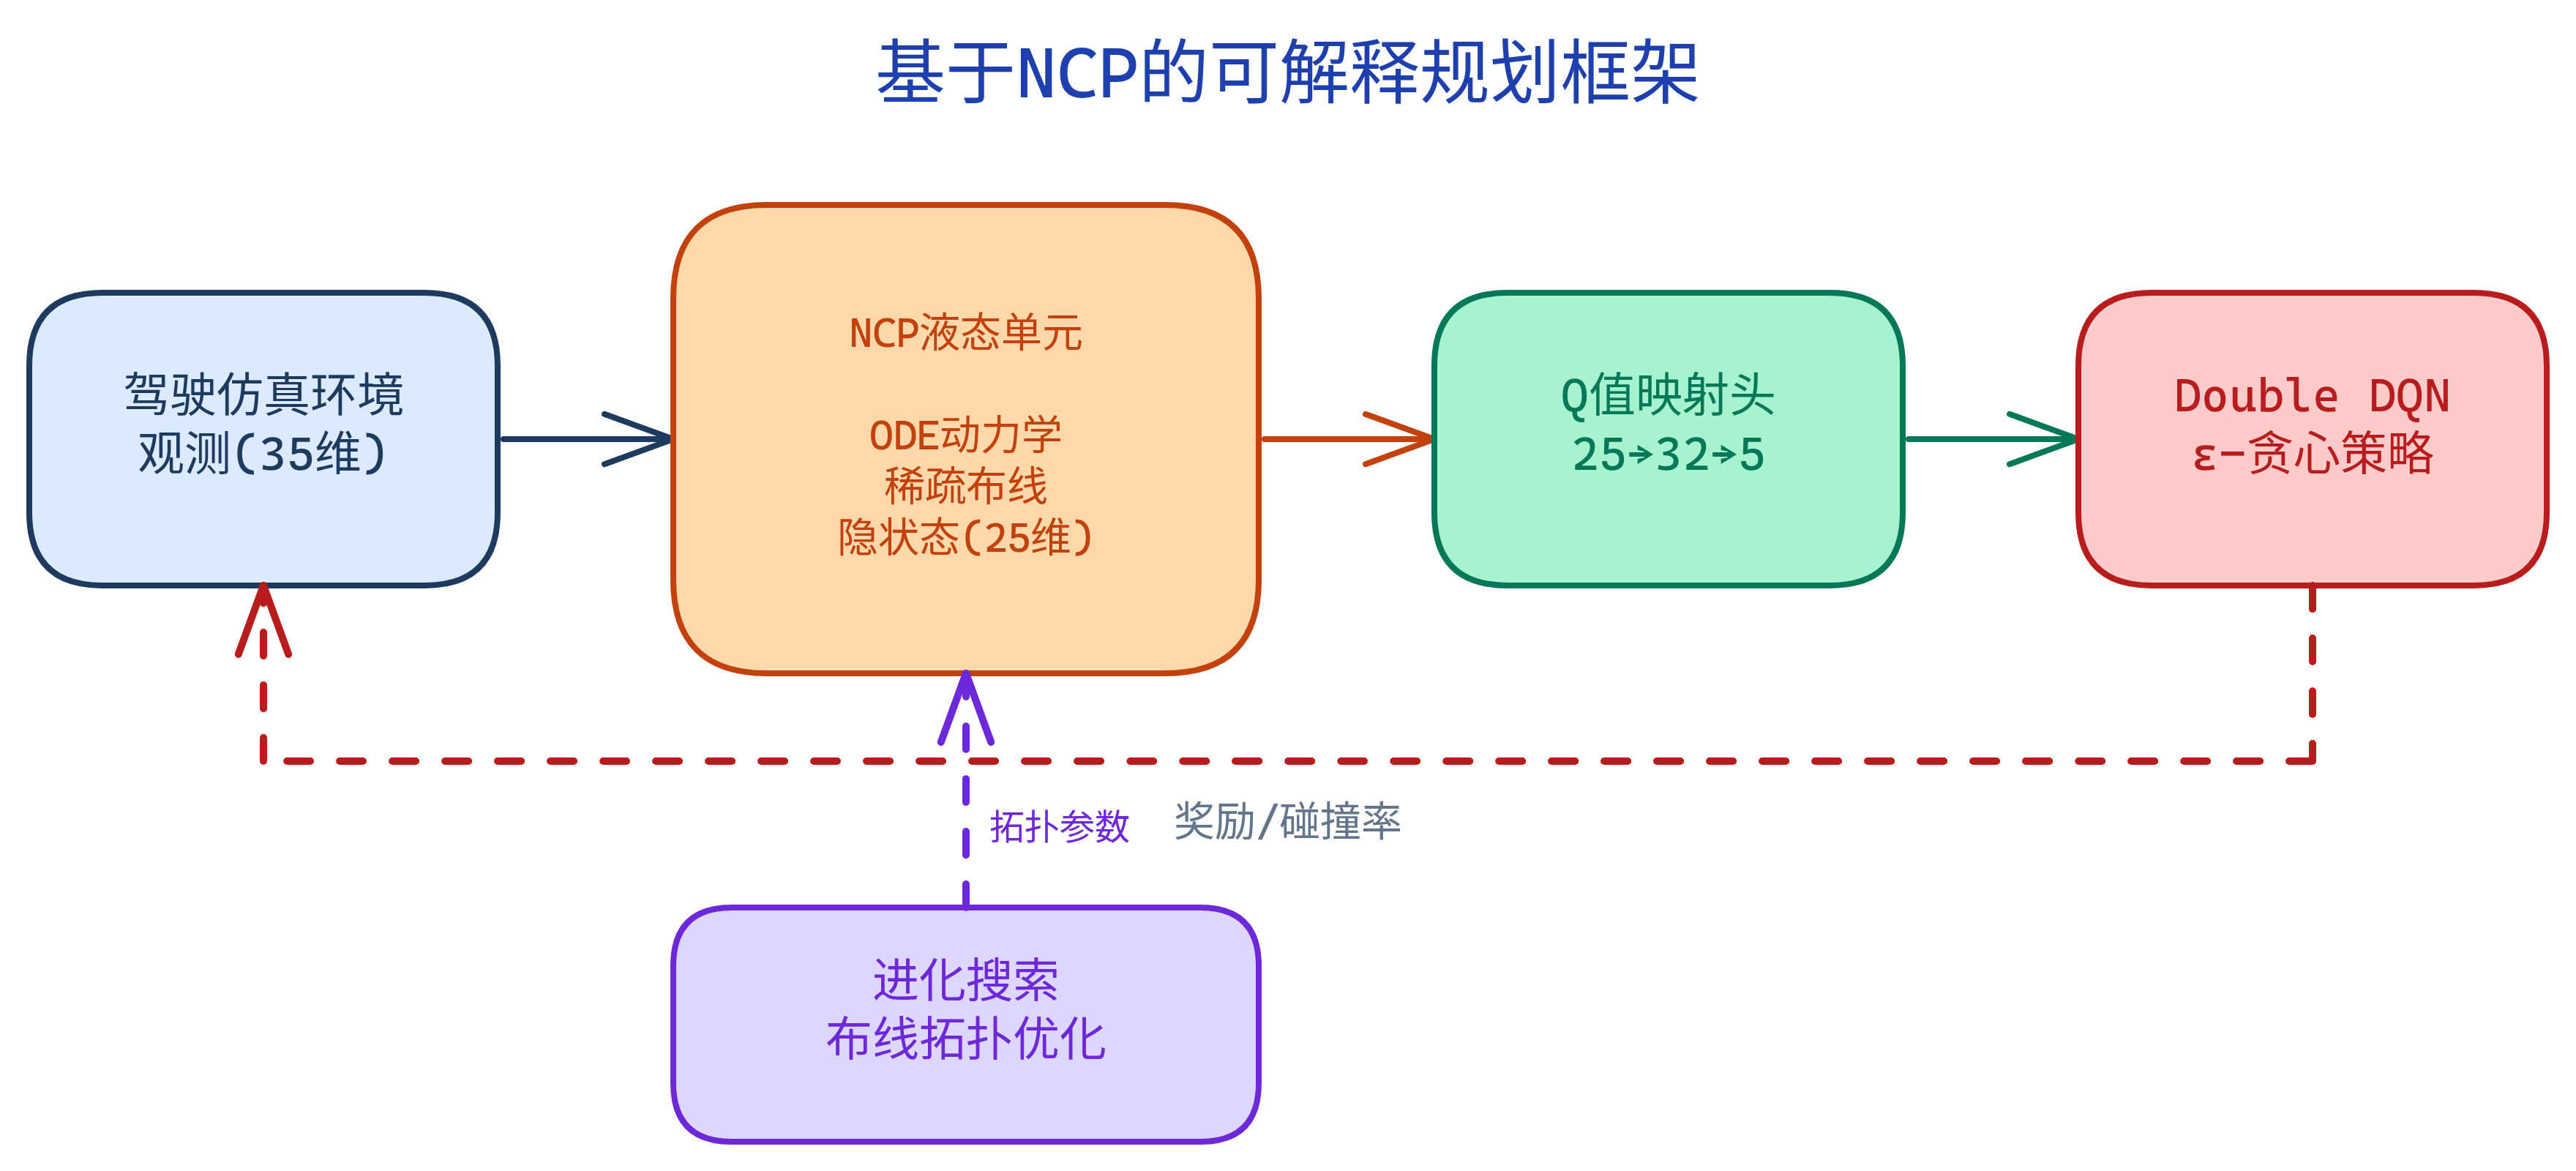
\includegraphics[width=0.9\linewidth]{img/fig_framework.png}
    \caption{基于NCP的可解释规划框架}
    \label{fig:framework}
\end{figure}

算法\ref{alg:framework}给出了本文方法的整体训练流程。

\begin{algorithm}[H]
\caption{基于NCP的可解释规划训练流程}
\label{alg:framework}
\begin{algorithmic}[1]
\Require 驾驶环境 $\mathcal{E}$，训练步数 $T$，搜索代数 $G$，种群大小 $N$
\Ensure 训练后的 NCP Q 网络 $Q_\theta$ 与最优布线拓扑 $g^*$

\State \textit{// 阶段一：进化搜索最优布线拓扑}
\State 随机初始化布线基因组种群$\mathcal{P}_0 = \{g_1, \ldots, g_N\}$
\For{$gen = 1$ to $G$}
    \For{每个基因组$g_i \in \mathcal{P}_{gen}$}
        \State 根据$g_i$构建NCP布线，实例化Q网络
        \State 在$\mathcal{E}$上快速训练$T_{\text{fit}}$步
        \State 计算适应度$F(g_i) = \bar{R}(g_i) - \alpha \cdot \bar{C}(g_i)$
    \EndFor
    \State 精英保留，锦标赛选择父代
    \State 交叉、变异、约束修复生成下一代$\mathcal{P}_{gen+1}$
\EndFor
\State $g^* \gets \arg\max_g F(g)$

\State \textit{// 阶段二：基于最优拓扑的完整训练}
\State 根据$g^*$构建NCP布线，实例化LTC单元和两层Q-head
\State 初始化在线网络$Q_\theta$、目标网络$Q_{\theta^-}$、经验回放缓冲区$\mathcal{D}$
\For{$t = 1$ to $T$}
    \State 以$\varepsilon$-贪心策略采样动作$a_t$，执行并存储$(s_t, a_t, r_t, s_{t+1})$到$\mathcal{D}$
    \State 从$\mathcal{D}$采样长度为8的序列，计算Double DQN目标
    \State 反向传播更新$\theta$，对NCP参数执行$w, c_m, g_{leak} \geq 0$裁剪
    \State 线性衰减$\varepsilon$；每500步更新$\theta^- \gets \theta$
\EndFor
\State \Return 训练后的$Q_\theta$与$g^*$
\end{algorithmic}
\end{algorithm}

该框架的设计理念是\textbf{分层解耦}：NCP负责时序动力学建模（液态ODE），Q-head负责值函数逼近（标准MLP），训练算法负责稳定优化（Double DQN），搜索算法负责结构优化（进化策略）。各模块各司其职，可独立替换和分析。
